\section{Grundlagen}
In diesem Kapitel wird der mathematische Hintergrund des Maschinellen Lernens beschrieben.
Zur Veranschaulichung wird die Problemstellung der Bachelorarbeit benutzt, bei der es darum geht, Ziffern einer Sieben-Segment-Anzeige zu erkennen.

\subsection{Maschinelles Lernen}
Beim Maschinellen Lernen geht es darum, dass der Computer aus  zur Verfügung gestellten Datensätzen selbstständig Muster und Regeln erkennt. \cite{Matzka_2021}

Es wird also kein Programm mehr geschrieben,  mit dem in unserem Beispiel genau beschrieben werden muss,  wie genau die verschiedenen Ziffern erkannt und differenziert von einander werden.
Stattdessen wird ein Algorithmus geschrieben, der an Hand von Daten sich selbstständig aktualisiert und lernt. Dies wird als Modelltraining bezeichnet.\\
Mit dem abgeschlossenen Modell können Vorhersagen über neue Daten getroffen werden.  So kann das Modell zur Ziffernerkennung aus einem Bild einer Eins bestimmen,  mit welcher Wahrscheinlichkeit es sich bei der Ziffer um eine Eins handelt.\\
Es gibt drei Hauptrichtungen des Maschinellen Lernens: Überwachtes Lernen,  Unüberwachtes Lernen und Verstärktes Lernen.
%\begin{figure}[h]
%\centering
%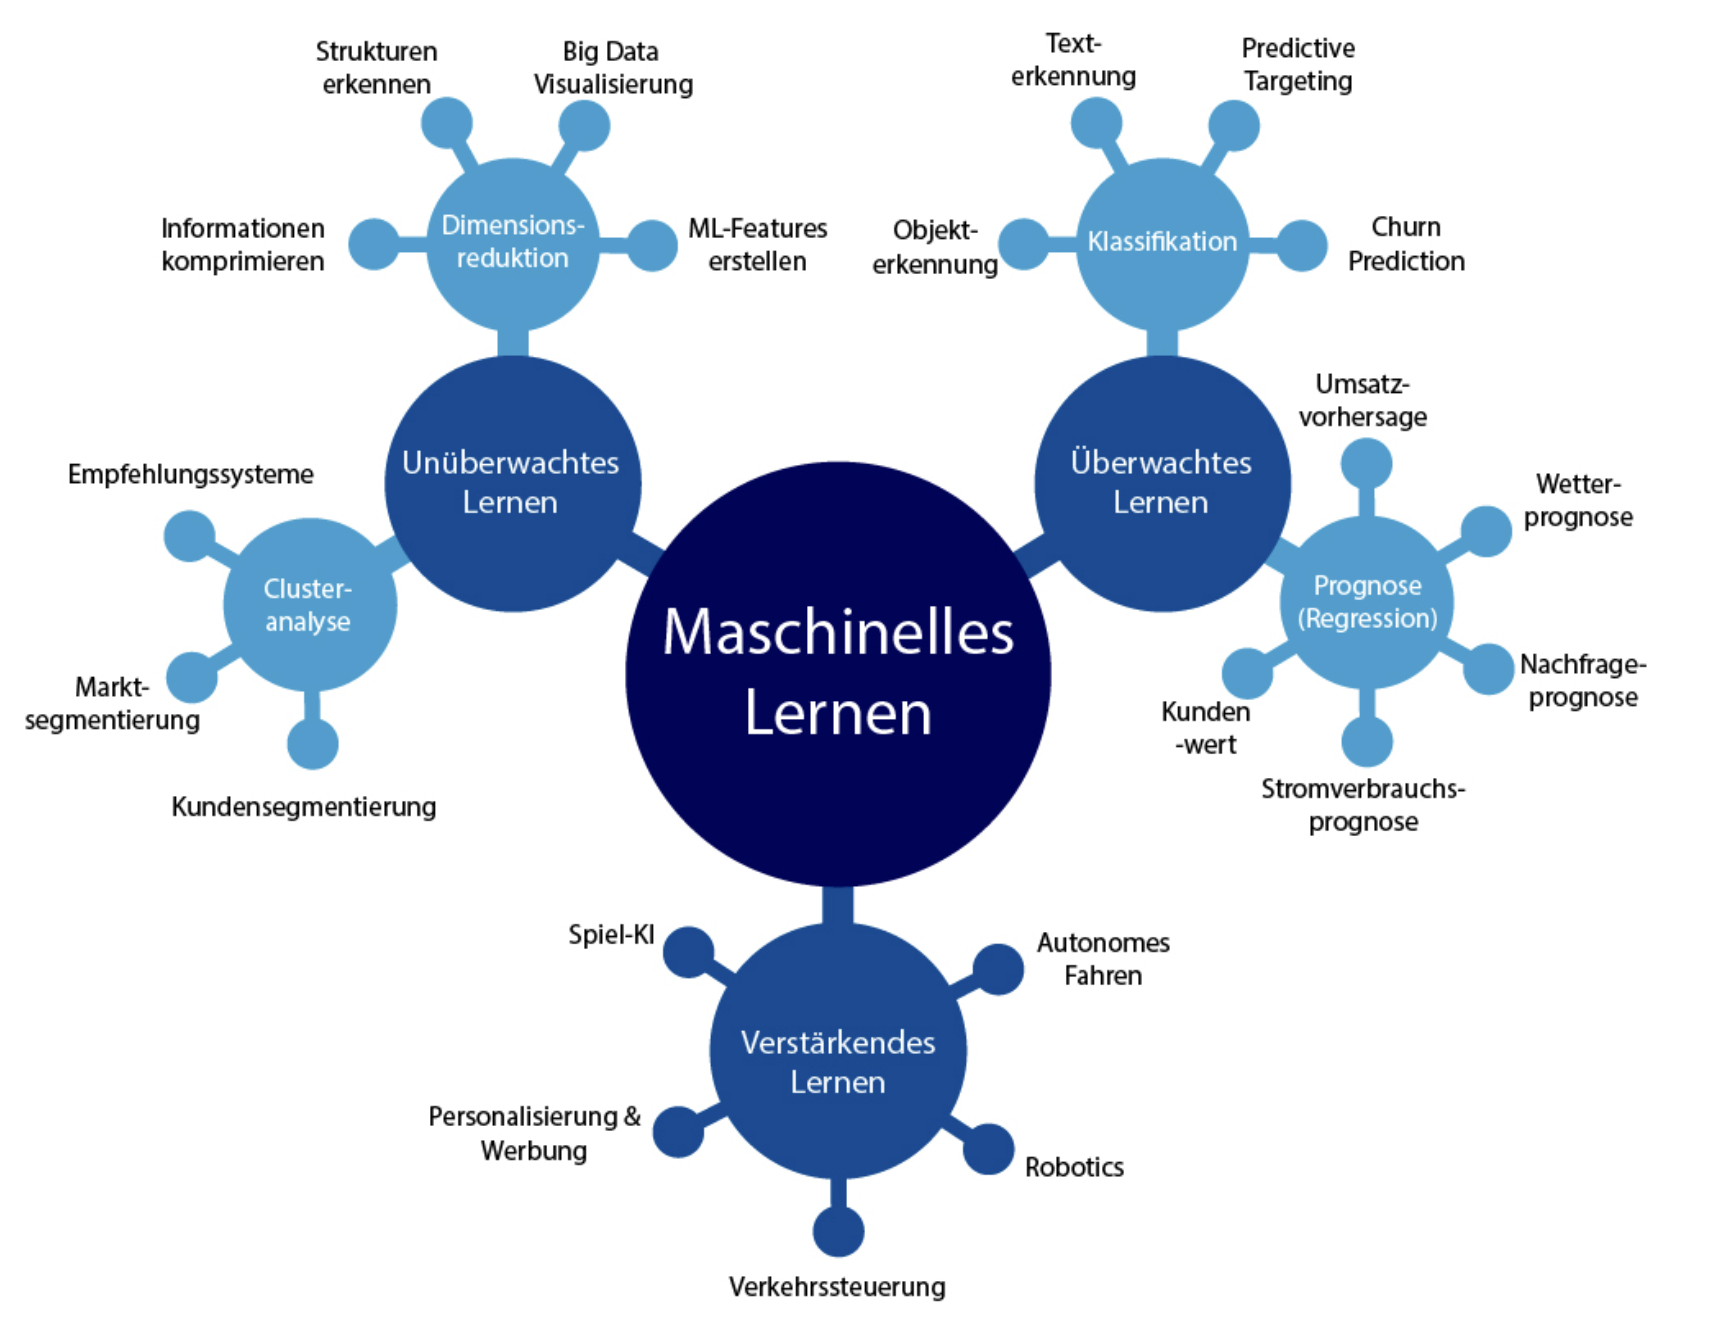
\includegraphics[scale=0.5]{pic/ML-Uberblick}
%\caption[ML-Uberblick]{Überblick Maschinelles Lernen}
%\end{figure}
Bei dem Überwachten Lernen wird mit einem bekannten Datensatz und auch vorgebenen Zielvariablen gelernt.  Es soll der Zusammenhang zwischen den beiden Werten  gelernt werden und richtig prognostiziert werden.  Diese Art von Maschinellem Lernen wird in dieser Arbeit verwendet.\\
Beim Unüberwachtem Lernen bekommt der Algorithmus Daten, aber keine Zielvariablen und muss die Daten selbst in Gruppen oder Muster einteilen.\\
Beim Verstärktem Lernen interagiert der Algorithmus mit der Umgebung und es gibt ein Belohnungssystem.  So entwickelt der Algorithmus selbstständig Lösungen zu einem Problem.\cite{url:datasolut.com-20210901}\\
Im weiterem wird sich nur noch auf das Überwachte Lernen bezogen.

\subsection{Arbeitslauf}
In einem Projekt zum Maschinellen Lernen (ML)  wird sich damit beschäftigt, welche Merkmale der Daten wichtig für die Fragestellung sind.  In dieser Bachelorarbeit soll eine Sieben-Segment-Anzeige erkannt werden. Dazu müssen möglichst viele verschiedene Daten von dieser Anzeige erhoben  und mit einem Label versehen werden.  Das Label ist die Zielvariable,   nach der Algorithmus unterscheiden soll,  in diesem Fall nach den Ziffern Null bis Neun. 
\begin{figure}[h]
\centering
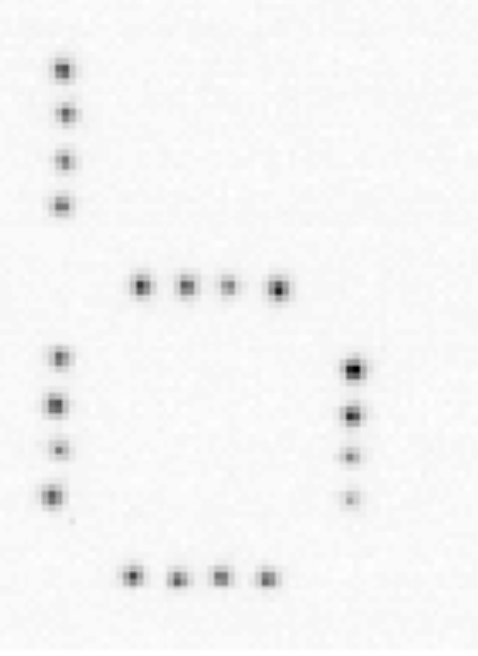
\includegraphics[scale=0.5]{pic/sechs}
\caption[Sechs]{Aufnahme mit der Sieben-Segment-Anzeige mit Label: 6}
\end{figure}
Nachdem Erheben der Daten werden diese visualisiert und analysiert. \\
Im nächsten Schritt werden die Daten für den ML Algorithmus vorbereitet, dazu gehört auch die Aufteilung der Daten und bereinigt.  Die Unterteilung erfolgt in drei Stücke, sogenannte Sets.
\begin{figure}[h]
\centering
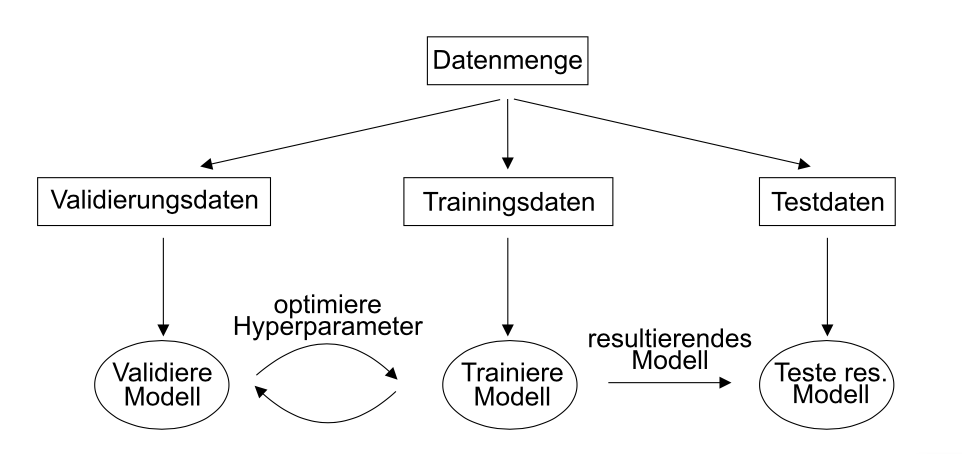
\includegraphics[scale=0.8]{pic/ML-Arbeitsablauf}
\caption[ML-Arbeitsablauf]{Arbeitsablauf Maschinelles Lernen}\cite{Choo_2020}
\end{figure}

Die Daten werden in Trainings-, Test- und Validierungssets getrennt.  Der Algorithmus wird anhand der Trainingsdaten trainiert. Dieses Set sollte ungefähr 70 \% des gesamten Datensatzes beinhalten mit gleicher Verteilung von allen Zielvariablen.  \cite{Geron2019}\\
Das Testset wird benutzt, um die Qualität des Models zu beurteilen. Dieses Set sollte ungefähr 20 \% des Datensatzes beinhalten. Hierbei ist es wichtig,  dass der Algorithmus die Daten nicht zum Lernen benutzt. \\
Mit dem Validierungsset, welches 10 \% der Daten enthält,  werden später die Hyperparameter (z.B.  die Lernrate oder das Gewicht) des Models angepasst.  Zusätzlich wird es verwendet,  um eine Überanpassung (engl.:  Overfitting) zu verhindern. Beim Overfitting lernt der Algorithmus des Modells zu viele der spezifischen Kleinigkeiten des Trainingssets und ist nicht mehr so gut beim Generalisieren. Dieses fällt normalerweise bei dem Evaluieren des Modelles mit dem Validierungsset auf. Das Validierungsset wird beim Lernen gar nicht verwendet, dadurch kann der Algorithmus nicht seine besonderen Merkmale trainieren. Zusätzlich ist die Erkennungsrate gering, wenn der Algorithmus sich zu sehr spezialisiert hat.


\subsection{Überwachtes Lernen}
Der generelle Gedanke hinter dem Überwachten Lernen ist es, mit den vorhandenen Eingabedaten und Zielvariablen eine Schätzfunktion aufzustellen.  Diese Schätzfunktion mit Parametern untersucht wie von den Eingabedaten auf die Zielvariabeln geschlossen werden kann.  Die Parameter der Schätzfunktion werden in dem Lernprozess des Algorithmus anpasst um die Schätzfunktion zu verbessern.  Dazu wird eine Verlustfunktion aufgestellt.  Diese quantifiziert  die Güte der Schätzfunktion. Also wird beschrieben, wie groß die Abweichung der Schätzfunktion und der Zielvariable ist. Zur Optimierung der Schätzfunktion müssen ihre Parameter angepasst werden, dazu wird die Minimierung der Verlustfunktion benutzt.\\
Im Überwachten Lernen ist zwischen zwei Arten von Aufgaben zu unterscheiden: der Klassifikation und der Regression.  Die Regression versucht aus vorhanden Daten eine Vorhersage oder einen Rückschluss zu treffen.  Ein Beispiel wäre,  aus Wetterdaten das morgige Wetter vorherzusagen.  \\
Bei der Klassifikation gibt es diskrete Zielvariable und es soll ein neues Eingabeereignis in die Klassifikationskategorien einsortiert werden,  z.B das Erkennen von Straßenschildern. Dieses ist auch das Ziel dieser Arbeit. So sollen in einem neuen Eingabebild die Ziffer erkannt werden.\\
Es gibt verschieden Methoden und Algorithmen die bei dem Überwachten Lernen verwendet werden.  Die einfachste ist eine lineare Methode.  Diese wird hier einmal vorgestellt,  um die mathematischen Hintergründe zu erläutern.

\subsubsection{Lineare Klassifikation}
Bei der Linearen Klassifikation liegen Paare von Eingabewerten und Zielvariablen vor.  Als Beispiel sind in dieser Arbeit die Eingabewerte ein Vektor,  der das Bild beschreibt.  Jedes Pixel hat einen Eintrag für den Helligkeitswert von 0-255.  Die Zielvariablen haben die Werte der Ziffern von Null bis Neun. \\
\[{(x_{1} , y_{1}),  \dotso , (x_{m}, y_{m})}\]
Bei der Klassifikation wird normalerweise eine Kodierung verwendet statt einfach die natürlichen Zahlen zu nutzen, da diese eine Ordnung untereinander besitzen und der Algorithmus diese erlernen könnte.\\
Eine Art von Kodierung ist die \emph{One-Hot-Kodierung} dabei wird die Zielvariable zum Einheitsvektor in diese Richtung \cite{Choo_2020}.
\begin{equation}
y \rightarrow e^{(y)} = 
\begin{bmatrix}
e_{1}^{(y)} \\
 \vdots\\
  e_{y}^{(y)}\\
   \vdots \\
    e_{p}^{(y)} \\ 
\end{bmatrix} 
=
 \begin{bmatrix}
 0\\
  \vdots \\
   1 \\
    \vdots \\
     0 \\
\end{bmatrix}
\end{equation}
Der Vektor der Eingabewerte \[x^{T} = (x_{1}, x_{2}, \cdots, x_{n})\] und der Parameter $\beta$ bilden eine lineare Schätzfunktion:\\
\begin{equation}
f(x|\beta) = \beta_{0} + \sum_{ j= 1}^{n} \beta_{j} x_{j} =\tilde{x}^{T}
\end{equation}\\
mit \[\tilde{x}^{T} = (1,x_{1}, \cdots, x_{n})\] \\ und \[ \beta = (\beta_{0}, \cdots, \beta_{n})\] \\
Um den Parameter $ \beta$ zu optimieren wird eine Verlustfunktion minimiert.\\
\begin{equation}
\beta_{opt} = argmin L(\beta)
\end{equation}\\
Das Minimierungsproblem ist in der Mathematik gut und viel erforscht, deswegen gibt es für ML verschiedene Verlustfunktionen.  
Hier wird die Verlustfunktion der Quadratsumme der Residuen (RSS) beschrieben.  RSS wird auch als L2-Verlust oder Gauß-Verlust bezeichnet. Sie gibt einen Abstand zwischen dem Ergebnis der Schätzfunktion und der Zielvariable an.  \\
\begin{equation}
\text{RSS}(\beta) = \sum_{i= 1}^{m} [y_{i} - f(x_{i}|\beta)]^{2}
\end{equation}\\
\begin{comment}
Um das Ganze als Matrixgleichung auszudrücken, werden die Eingabedaten zu einer $(m \times (n+ 1)$ Matrix mit Einträgen $x_{i}^{T}$ und den Zielvariablen zum Vektor $Y^{T} = (y_{1}, \cdots, y_{m})$:
\begin{equation}
\text{RSS}(\beta) = (Y- \tilde{X}\beta)^{T})(Y- \tilde{X}\beta)
\end{equation}\\
Das Minimum der Funktion wird über die Nullstellen der partiellen Ableitung erster Ordnung und eine positive partielle Ableitung zweiter Ordnung definiert. Wenn $\tilde{X}^T\tilde{X}$ einen Vollrang (gleiche Zeilen- und Spaltenanzahl) hat und damit invertierbar ist,  so ist die Lösung \cite{Choo_2020}:
\begin{equation}
\beta = (\tilde{X}^T\tilde{X})^{-1} (\tilde{X}^T\tilde{X})
\end{equation}
\end{comment}
Für die Einordnung eines neuen Eingabewertes in eine Klasse wird,  nach dem  das Optimieren der Schätzfunktion abgeschlossen ist,  eine Aktivierungsfunktion benutzt.  Sie gibt die Wahrscheinlichkeit,  dass die Eingabewerte einer Klasse angehören an.  Dabei wird das größte Element aus dem Ergebnisvektor der Schätzfunktion gesucht:
\begin{equation}
F(x|\beta) = argmax_{k} f_{k}(x|\beta)
\end{equation}
\subsection{Neuronale Netzwerke}
Die Grundidee der Neuronalen Netzwerke beruht auf dem Prinzip von biologischen Nervenzellen (Neuronen).  Es wird ein Eingangssignal verarbeitet und erst wenn ein Grenzwert überschritten wird,  folgt die Weiterleitung eines Impulses.\\
Bei einem Neuronalen Netzwerk werden die Eingangswerte mit einer Gewichtung belegt und innerhalb des Neurons aufsummiert.  Die Summe wird dann gegen einen Grenzwert überprüft und gegebenenfalls weitergeleitet \cite{Matzka_2021}.
\begin{figure}[h]
\centering
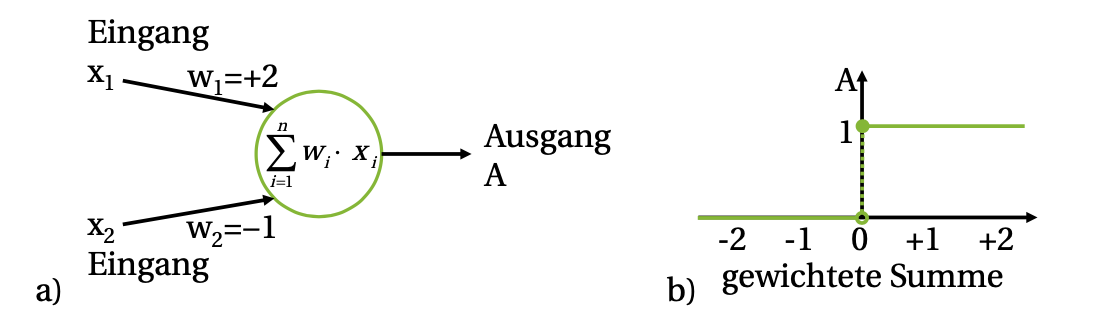
\includegraphics[scale=0.5]{pic/Neuron}
\caption[Neuron]{Neuron}\cite{Matzka_2021}
\end{figure}\\
Zur Vereinfachung wird in der Formel der Grenzwert auf die Seite der Eingangswerte ( $x_{i}$)  und Gewichte ($w_{i}$) geholt.  Der Grenzwert wird dann als Bias (b) bezeichnet und gehört mit den Gewichten zu den veränderbaren Parameter während des Trainierens des Netzwerkes. \cite{url:neuralnetworksanddeeplearning.com-2021}\\
\begin{equation} \label{linFunc}
\text{Ausgang} = \sum_{i=1}^{n} x_{i}w_{i} + b
\end{equation}
In einem Neuronalen Netzwerk werden mehrere Neuronen in eine Schicht gebaut und dann mehre Schichten hintereinander verknüpft.  Die Schichten zwischen den Eingabe- und Ausgabeschichten werden 'verdeckte Schichten' (engl. hidden Layers) genannt. \\
\begin{figure}[h]
\centering
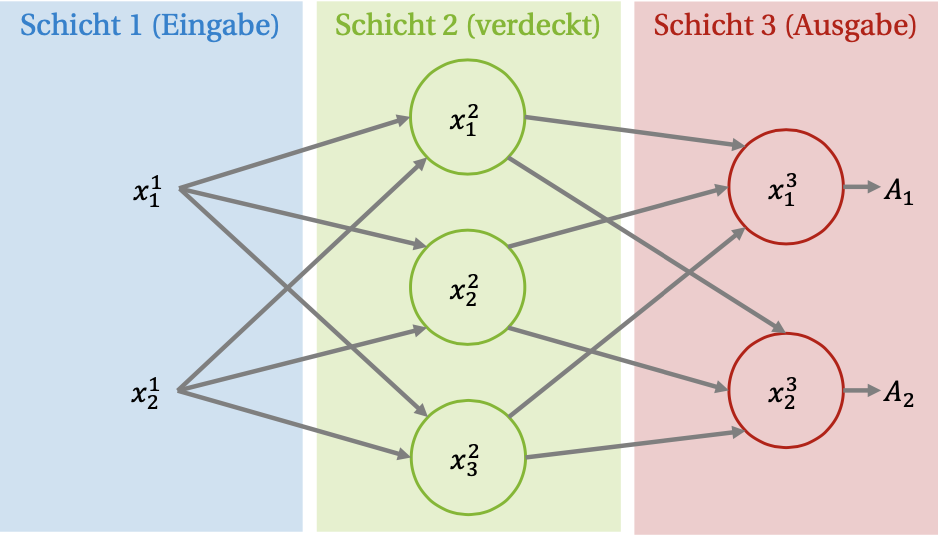
\includegraphics[scale=0.6]{pic/Netzwerk}
\caption{Netzwerk Aufbau}\cite{Matzka_2021}
\end{figure}\\
In dem Netzwerk werden alle Neuronen einer Schicht mit allen Neuronen in der nächsten Schicht verbunden.  Jede dieser Verbindungen hat ihr eigenes Gewicht und die Neuronen haben jeweils eine Bias \cite{Matzka_2021}.
\begin{figure}[h]
\centering
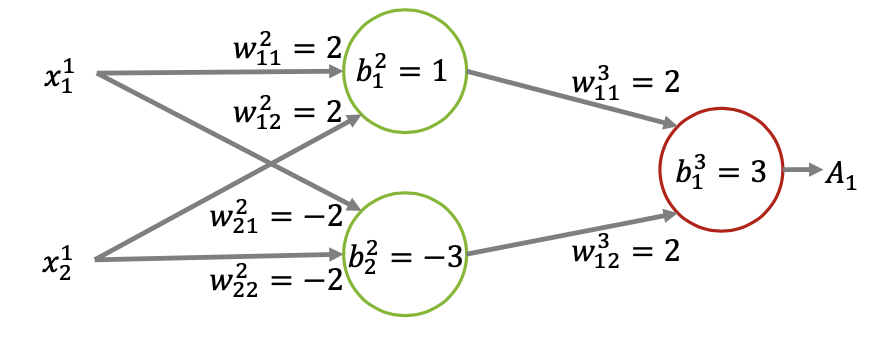
\includegraphics[scale=0.8]{pic/NeuronFormel}
\caption{ Neuronen in mehrschichtigen Netzwek}\cite{Matzka_2021}
\end{figure}\\
\subsubsection{Aktivierungsfunktion}
Bei der Gleichung \ref{linFunc} handelt es sich um eine lineare Funktion.  Für Neuronale Netzwerke werden nicht-lineare Funktionen als 'Aktivierungsfunktionen' benutzt,  da sie besser als lineare Funktionen geeignet sind,  unterschiedliche Gewichtungen bei den Eingabewerten abzufangen.  Es wird versucht  Funktion als Aktivierungsfunktion zu benutzten. Diese haben den Vorteil, dass es beim Lernen, wo differenziert wird,  nicht zu Lücken kommt.  Außerdem können Funktionen mit begrenzten Wertebereich hilfreich sein. So können zu große Eingabewerte nicht zu extrem Ergebnissen der Aktiierungsfunktion führen  \\
Aktivierungsfunktionen \cite{Choo_2020}:\\
\begin{tabular}{lp{10cm}}
\textbf{ReLu: }& rectified linear unit, alle negativen Zahlen verschwinden,  während es eine linear wachsende Funktion für positive Zahlen ist\\
 & \\
\textbf{Sigmod: }& eine geglättet Version der Stufenfunktion\\
 & \\
\textbf{Hyberbolische Tangens: } & ähnliches Verhalten wie Sigmod, kann aber für positive und negative Werte annehmen\\
 & \\
\textbf{Softmax: } & often für die letzte Schicht bei Klassifikationsaufgaben verwendet\\
\end{tabular}
\\
\begin{figure}[h]
\centering
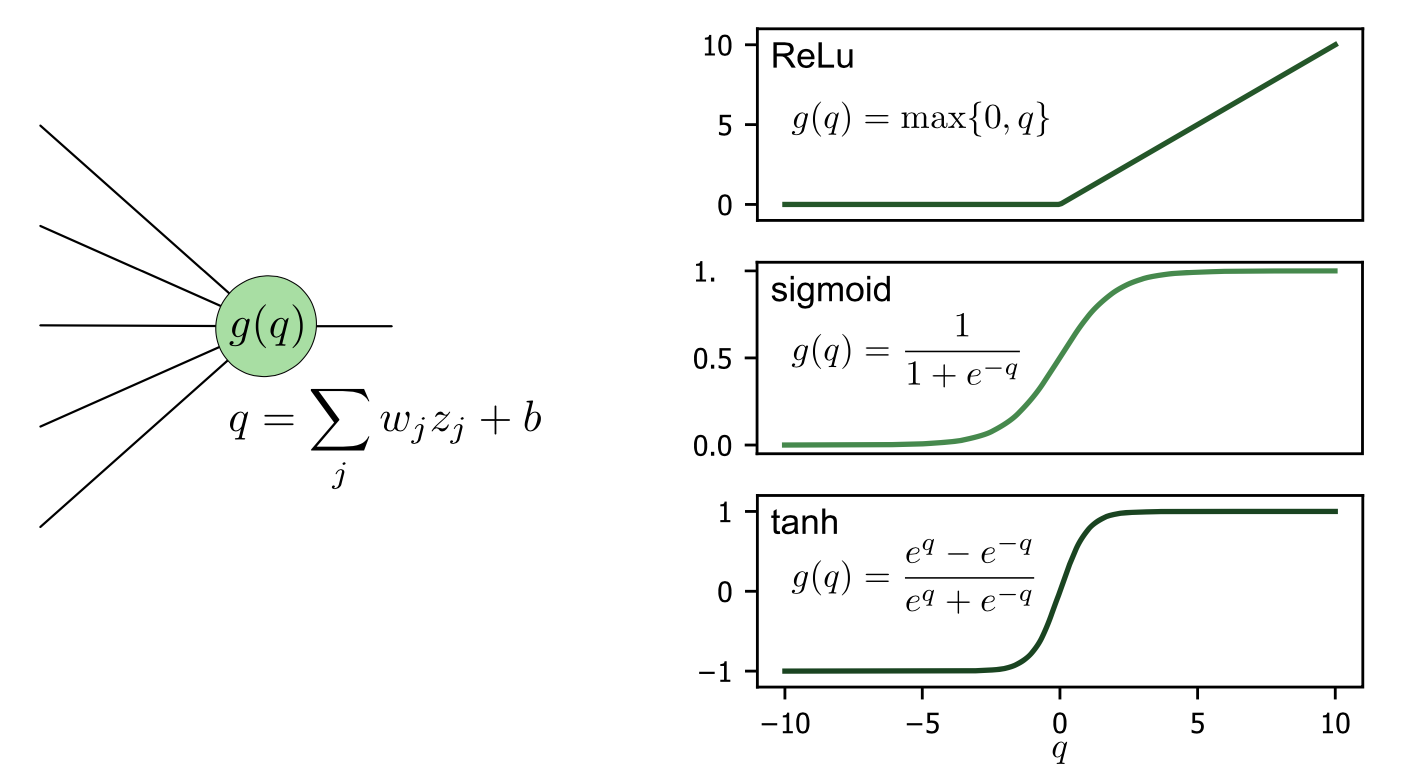
\includegraphics[scale=0.5]{pic/Aktivierungsfunktion}
\caption[Aktivierungsfunktion]{Aktivierungsfunktion \cite{Choo_2020}}
\end{figure}
%Berechnung nochmals erklären mit Beispiel
\subsubsection{Training}
Bei dem Training von Neuronalen Netzwerken werden die Parameter Gewichte und Bias optimiert.  Hierzu wird auch eine Verlustfunktion benutzt.  Diese ist abhängig von den Parameter Gewicht (w) und Bias (b). 
\begin{equation}
 L(w, b)= \frac{1}{n} \sum_{i =1}^{n} \lVert F(x_{i})-z_{i} \rVert^{2}
\end{equation}
Dies ist die Verlustfunktion des mittleren absoluten Fehlers mit $F(x)$ der Schätzfunktion und z der Zielvariablen.  Bei $\lVert a \rVert$ handelt es sich um die Norm,  die Länge des Vektors.  Eine alternative Verlustfunktion, gerade für Klassifikationsaufgaben, ist die Kreuzentrophie: \\
\begin{equation}
L_{cross}(w,b)= - \sum_{i=1}^{m} y_{i} \cdot ln(F(x_{i}))
\end{equation}
Das Ziel ist es, die Verlustfunktion zu minimieren,  also den Abstand zwischen dem Ergebnis der Schätzfunktion und der Zielvariablen möglichst klein zu bekommen.\\
\subsubsection{Gradientenabstieg} \label{Gradient}
In Neuronalen Netzwerken ist die Verlustfunktion normalerweise hochdimensional und kann meistens nicht analytisch gefunden werden.  Da nummerische Verfahren extrem aufwendig sind,  wird meistens nur nach einem lokalen,  anstelle eines globalen Minimums gesucht. \\
Dazu wird der Gradient gebildet und so die Richtung bestimmt,  in welche die Parameter $w$ und $b$ verändert werden sollen.  Diese wird in kleinen Schritten, der Lernrate $\eta$, wiederholt.
\begin{equation}
(w_{ij},b_{i}) \rightarrow (w_{ij},b_{i}) - \eta \frac{\delta L_{w ,b}}{\delta (w_{ij},b_{i}})
\end{equation}
Man kann sich das Ganze vorstellen wie einen Ball, der immer wieder fallen gelassen wird und in die nächste  Kuhle rollt.  Dabei gibt es die Schwierigkeit, die richtige Größe der Lernrate $\eta$ zu finden.  Bei zu kleiner Lernrate $\eta$ kommt es nur zu kleinen Veränderungen der Modellparameter $w$ und $\beta$ (Abb.\ref{fig: Lernrate}. a). Ist aber die Lernrate $\eta$ zu groß,  so kann das lokale Minimum übersprungen werden und  der Algorithmus gerät in eine Schleife (Abb.\ref{fig: Lernrate} c).\\
\begin{figure}[h]
\centering
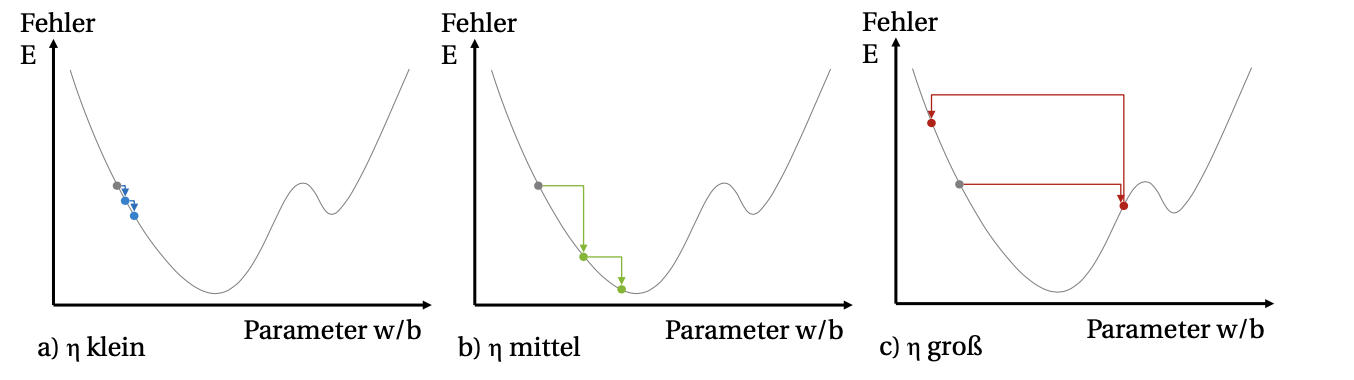
\includegraphics[scale=0.6]{pic/Lernrate}
\caption{Einfluss der Lernrate}\cite{Matzka_2021}
\label {fig: Lernrate}
\end{figure}
\subsubsection{Aufteilung in Batches}
Die Trainingsdaten werden normalerweise nochmals in sogenannte Batches (deutsch: Stapel) unterteilt.  Dieses wird getan,  damit nicht nach jeden Trainingspunkt die Modellparameter angepasst werden,  sondern immer erst,  nachdem ein gesamter Batch durchgelaufen ist. \\
Bei der Batch Unterteilung gibt es drei Hauptvarianten:
\begin{description}
\item[Batch Gradientenabstieg: ]Batch Größe = Größe des Traingingsets
\item[Stochastischer Gradientenabstieg: ] Batch Größe = 1
\item[Mini-Batch Gradientenabstieg: ] 1 < Batch Größe < Größe des Traingingsets
\end{description}
Die Batch Größe ist ein wichtiger Parameter bei Trainieren des Netzwerkes.  Auf der ein Seite ist die Rechenzeit, die ein Netzwerk zum Trainieren braucht, desto mehr Berechnung und Gradienten aufgestellt werden, desto länger dauert es.  Aber die Wahrscheinlichkeit das global Minimum zu finden steigt natürlich mit der Anzahl der Berechnung. 


